\documentclass[11pt,letterpaper]{article}
\usepackage[utf8]{inputenc}
\usepackage[left=1in,right=1in,top=1in,bottom=1in]{geometry}
\usepackage{amsfonts,amsmath}
\usepackage{graphicx,float}
\usepackage{esint}
\usepackage{csquotes}
% -----------------------------------
\usepackage{hyperref}
\hypersetup{%
  colorlinks=true,
  linkcolor=blue,
  citecolor=blue,
  urlcolor=blue,
  linkbordercolor={0 0 1}
}
% -----------------------------------
\usepackage[authordate,backend=biber]{biblatex-chicago}
\addbibresource{citation.bib}
% -----------------------------------
\usepackage{fancyhdr}
\newcommand\course{MATH-UA.0230, PHYS-UA 180\\Introduction to Fluid Dynamics}
\newcommand\hwnumber{6}                  % <-- homework number
\newcommand\NetIDa{Ryan Sh\`iji\'e D\`u} 
\newcommand\NetIDb{March 10th, 2023}
\pagestyle{fancyplain}
\headheight 35pt
\lhead{\NetIDa\\\NetIDb}
\chead{\textbf{\Large Worksheet \hwnumber}}
\rhead{\course}
\lfoot{}
\cfoot{}
\rfoot{\small\thepage}
\headsep 1.5em
% -----------------------------------
\usepackage{titlesec}
\renewcommand\thesubsection{(\arabic{section}.\alph{subsection})}
\titleformat{\subsection}[runin]
        {\normalfont\bfseries}
        {\thesubsection}% the label and number
        {0.5em}% space between label/number and subsection title
        {}% formatting commands applied just to subsection title
        []% punctuation or other commands following subsection title
% -----------------------------------
\setlength{\parindent}{0.0in}
\setlength{\parskip}{0.1in}
% -----------------------------------
\newcommand{\de}{\mathrm{d}}
\newcommand{\DD}{\mathrm{D}}
\newcommand{\pe}{\partial}
\newcommand{\mcal}{\mathcal}
%\newcommand{\pdx}{\left|\frac{\partial}{\partial_x}\right|}

\newcommand{\dsp}{\displaystyle}

\newcommand{\norm}[1]{\left\Vert #1 \right\Vert}
%\newcommand{\mean}[1]{\left\langle #1 \right\rangle}
\newcommand{\mean}[1]{\overline{#1}}
\newcommand{\inner}[2]{\left\langle #1,#2\right\rangle}

\newcommand{\ve}[1]{\boldsymbol{#1}}

\newcommand{\thus}{\Rightarrow \quad }
\newcommand{\fff}{\iff\quad}
\newcommand{\qdt}[1]{\quad \mbox{#1} \quad}

\renewcommand{\Re}{\mathrm{Re}}
\renewcommand{\Im}{\mathrm{Im}}
\newcommand{\E}{\mathbb{E}}
\newcommand{\lap} {\nabla^2}
\renewcommand{\div}{\nabla\cdot}

\newcommand{\csch}{\text{csch}}
\newcommand{\sech}{\text{sech}}


\newcommand{\hot}{\text{h.o.t.}}

\newcommand{\ssp}{\left.\qquad\right.}

\newcommand{\var}{\text{var}}
\newcommand{\cov}{\text{cov}}


\begin{document}

\section{Simple model for river flow}
[From \cite{Falkovich_18}, \S 1.4.3] 
We use a simple include plane as a model for river flow.
\begin{figure}[H]
    \centering
    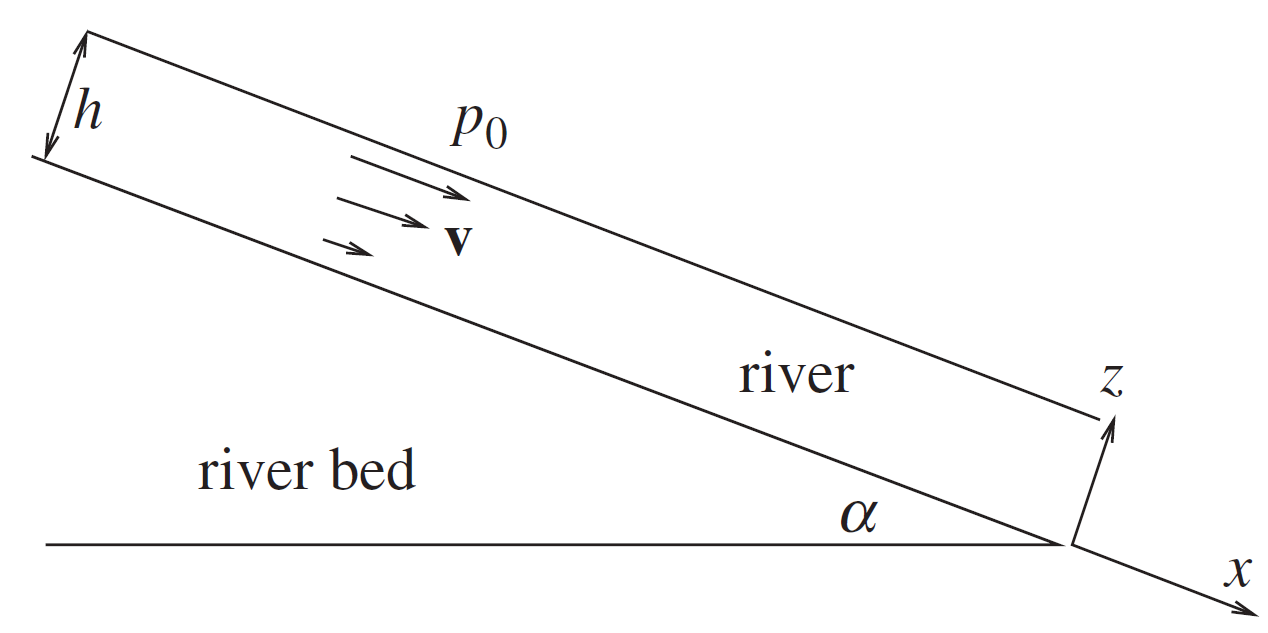
\includegraphics[width=0.55\textwidth]{figs/incline_river}
\end{figure}

\subsection{}
Assume we have a steady solution to the Navier-Stokes equation, show $(\ve v\cdot\nabla)\ve v = 0$. This implies we have an effectively linear equation
\begin{align}
    -\nabla p+\eta\nabla^2\ve v+\rho\ve g = 0.
\end{align}

Write the equation for the $x$ and $z$ direction defines in the figure.

\subsection{}
What should be boundary condition be for $v$ and $p$ at the surface and at the bottom? Solve for them.

\subsection{}
Take the kinematic viscosity of water to be $\nu = \eta/\rho = 10^{-2}\text{cm}^2\text{s}^{-1}$. Calculate $\ve v$ at the surface for a rain puddle with thickness $h = 1\text{mm}$ on a slope $\alpha\sim 10^{-2}$.

How about a slow plain rivers (like the Danube) with $h \sim 10\text{m}$ on a slope $\alpha\sim 10^{-4}$?

Which speed is reasonable?

\subsection{}
The unrealistic high velocity for the river case above is because in reality rivers are turbulent. 







% \section{}
% [From \cite{Aris_62}, Exercise 6.11.1] 




    
\vfill
\printbibliography


\end{document}